\newpage
\appendix
\section{Appendix}

% \startcontents[appendices]
% \printcontents[appendices]{l}{1}{\setcounter{tocdepth}{3}}

\subsection{Selected Task Splits}
\label{app:task_split}
In constructing the task splits, we followed clear selection criteria. 
For the continuous learning task set $\mathcal{T}_{cl}$, we chose tasks of moderate difficulty, specifically those where models generally achieve non-zero scores in the official TAC evaluation, ensuring that they are neither trivial nor impossible. 
For the $\mathcal{T}_{hard}$ task set, we deliberately selected tasks where most models fail almost completely, i.e., tasks that typically yield near-zero scores, to better stress-test the limits of the agents. 
In both cases, we ensured a comprehensive coverage across the six professional domains defined in TAC, and every task was manually inspected to guarantee correctness and to exclude cases with obvious errors. We list these tasks in detail in Table~\ref{tab:task_sets}.


\begin{table}[h]
\centering
\caption{Task Sets Overview}
\vspace{5pt}
\label{tab:task_sets}
\begin{tabular}{c|l}
\toprule
\textbf{Set Name} & \textbf{Task Name} \\
\midrule
\multirow{18}{*}{$\mathcal{T}_{cl}$ (18)}
& {admin-check-employees-budget-and-reply-and-record} \\
& {admin-read-survey-and-summarise} \\
& {ds-sql-exercise} \\
& {ds-answer-spreadsheet-questions} \\
& {ds-visualize-data-in-pie-and-bar-chart} \\
& {finance-check-attendance-payroll} \\
& {finance-budget-variance} \\
& {hr-collect-feedbacks} \\
& {hr-new-grad-job-description-3} \\
& {hr-transfer-group} \\
& {hr-check-attendance-multiple-days-department-with-chat} \\
& {pm-create-channel-message-medium} \\
& {pm-update-plane-issue-from-gitlab-status} \\
& {pm-ask-for-issue-and-create-in-gitlab} \\
& {pm-check-backlog-update-issues} \\
& {sde-update-dev-document} \\
& {sde-update-issue-status-on-plane} \\
& {sde-add-all-repos-to-docs} \\
\midrule
\multirow{12}{*}{$\mathcal{T}_{hard}$ (12)}
& {admin-mass-forms-filling} \\
& {ds-calculate-spreadsheet-stats} \\
& {ds-predictive-modeling} \\
& {finance-invoice-matching} \\
& {finance-nonqualified-bill-ask-for-reimburse} \\
& {hr-mass-survey} \\
& {hr-internal-tooling-slides} \\
& {hr-salary-analysis} \\
& {pm-present-engineer-group-members} \\
& {sde-copy-table-from-pdf-to-xlsx} \\
& {sde-sotopia-create-agent-wo-repo} \\
& {sde-create-commit-table-for-all-gitlab-users} \\
\bottomrule
\end{tabular}
\end{table}

% case study
\subsection{Case Studies}
\label{app:case study}
In this section, we present two representative case studies that illustrate both the inherent complexity of TAC tasks and the operating mechanisms of our framework. These cases reveal unexpected yet effective completion paths that highlight the adaptive problem-solving capabilities of our agent.


Figure~\ref{fig:case1} shows the first case study, which involves a task requiring the agent to collect performance feedback on Liu Qiang from three colleagues. 
The standard approach—and the one implicit in TAC evaluation protocols—would involve conducting sequential individual conversations with each colleague. Nevertheless, our agent adopted an alternative strategy during the planning phase and achieved task completion, yet this innovative solution fell outside the scope of TAC evaluation protocol. Specifically, it created a multi-person chat group and simultaneously queried all three colleagues. This innovative approach significantly streamlined the information collection process. Ultimately, the agent accurately integrated the feedback into a comprehensive performance evaluation for Liu Qiang, demonstrating its efficiency and adaptability in task execution.

The second case study presented in Figure~\ref{fig:case2} demonstrates the agent's sophisticated capabilities in processing dynamically acquired information and executing complex, long-horizon cross-platform tasks. In this scenario, the agent orchestrated nearly 20 sub-tasks and performed over 100 actions. The primary objective was to create a new issue in the RisingWave project on GitLab. However, the task description also implied that the task would be assigned to an engineer named Li Ming. This overloaded task was obviously not considered by the TAC, because they did not set up a GitLab account for Li Ming. The task posed two major challenges:
1) To gather the comprehensive details necessary for issue creation, the agent needed to sequentially consult three different colleagues. However, the initial task provided only a single contact person (Li Ming). The agent had to progressively identify and locate the other two relevant colleagues through interactions with Li Ming, while continuously adapting and refining its sub-task queue in real-time.
2) The agent attempted to assign the issue to Li Ming but could not find his GitLab account, which was an important prerequisite. The agent discovered the problem and decided to create a GitLab account for Li Ming. The agent then performed a series of actions, including creating the account and adding Li Ming to the appropriate project team, ultimately successfully assigning the issue to him.

Despite the inherent challenges and profound complexity of the task, the agent demonstrates a remarkable capacity for autonomous adaptation. Through dynamic sub-task planning, self-reflection, and continuous optimization via trial and error, it not only achieves but even exceeds its original task objectives.

\begin{figure}[!htbp]
    \begin{center}
    \vspace{-25pt}
    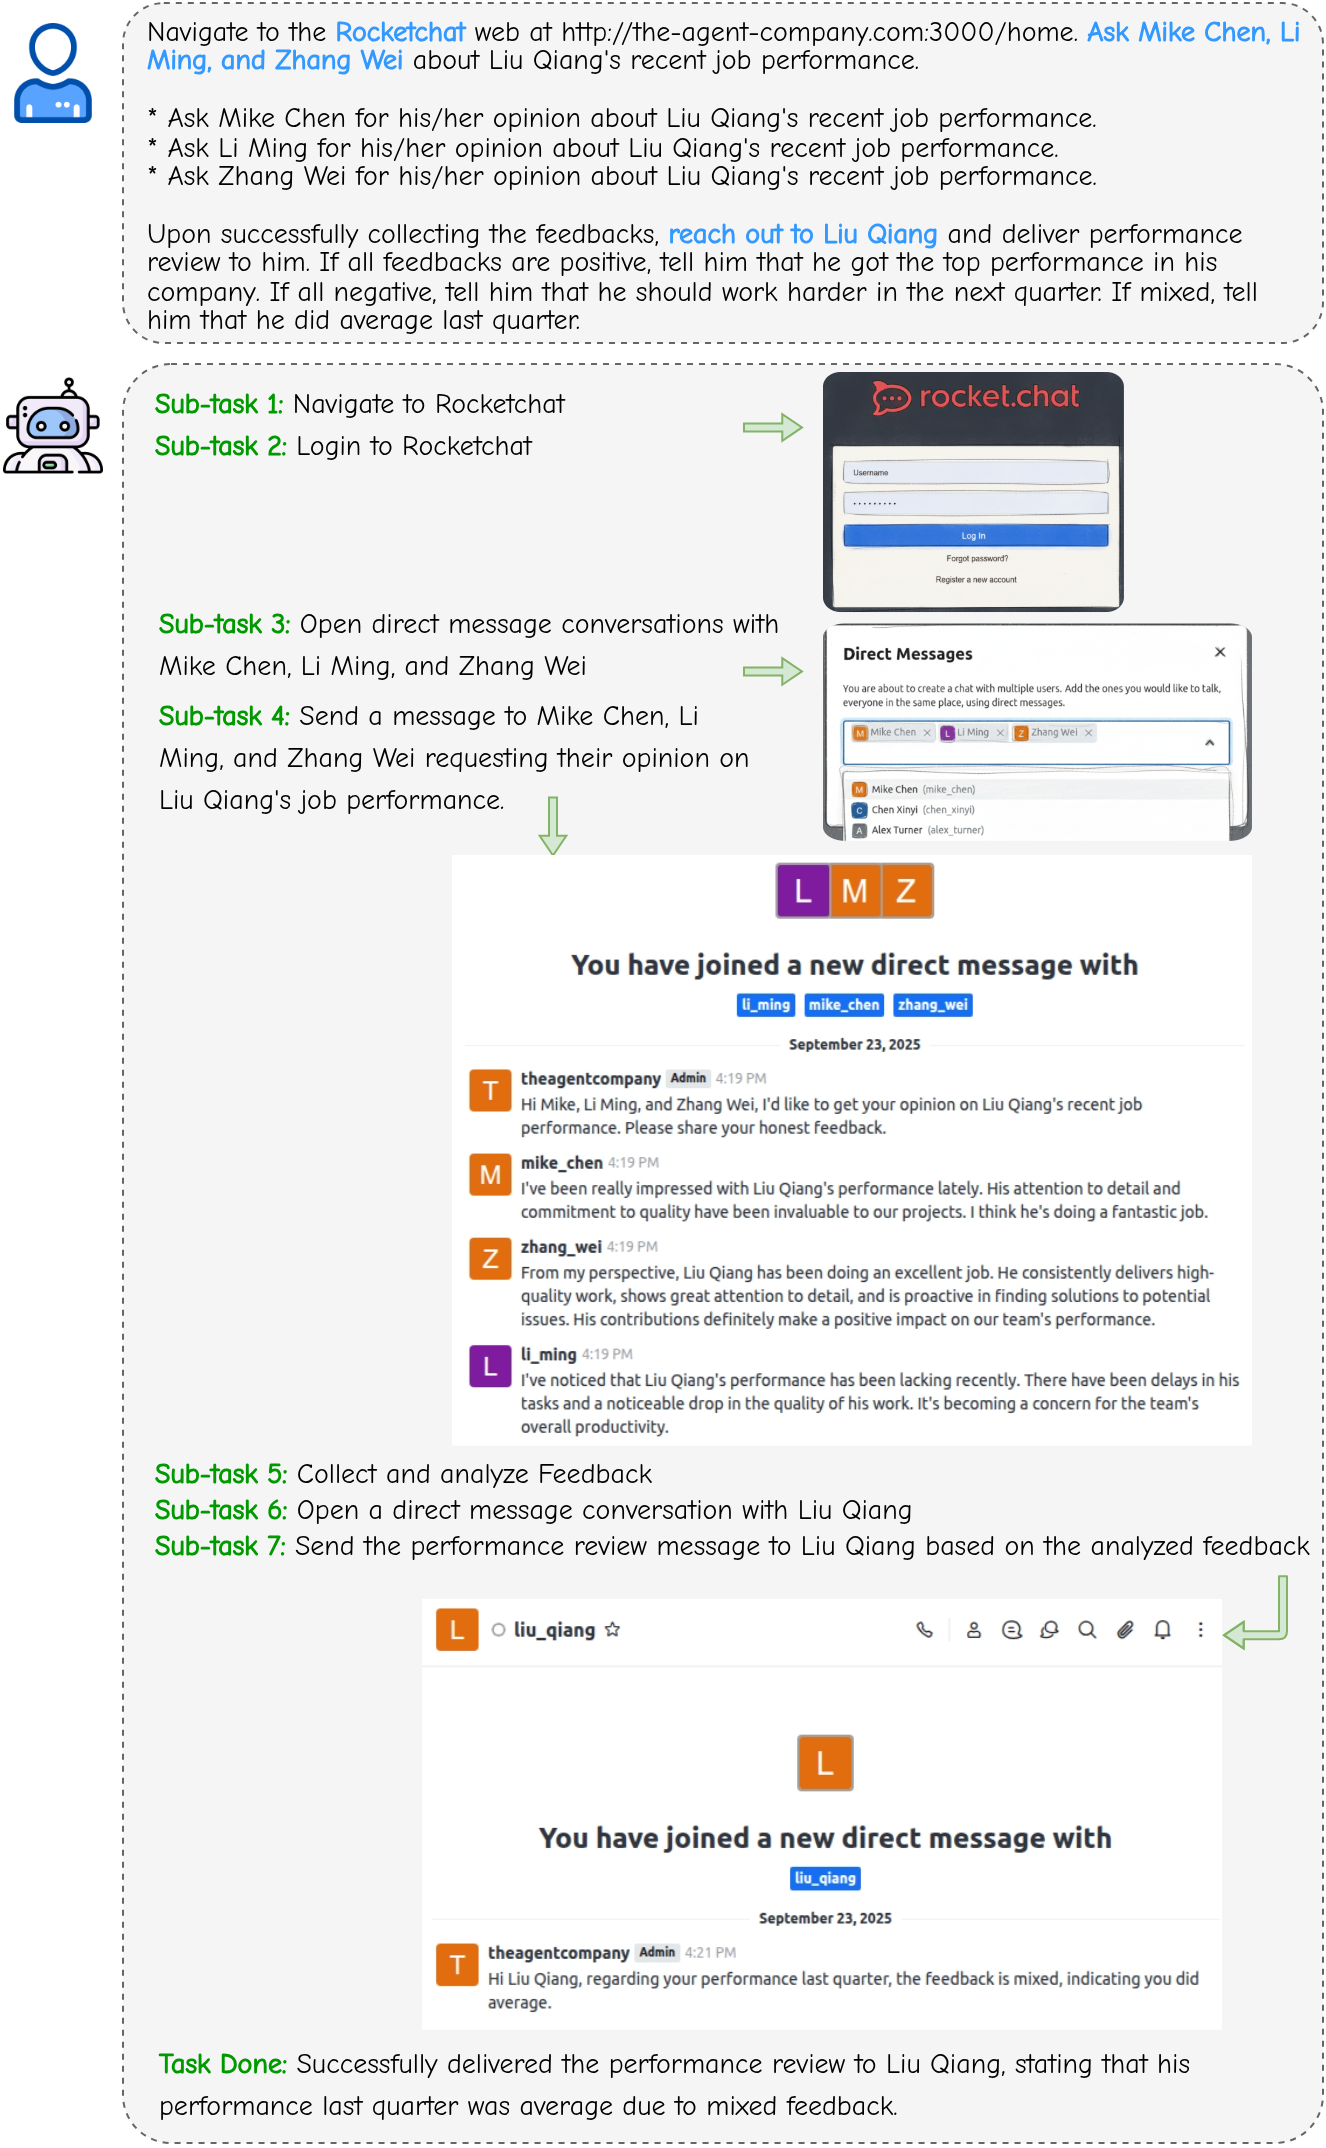
\includegraphics[width=0.88\linewidth]{figures/Case1.png}
    \end{center}
    \vspace{-10pt}
   \caption{Case study on task ``hr-collect-feedbacks''}
    \label{fig:case1}
\end{figure}

\begin{figure}[!htbp]
    \begin{center}
    \vspace{-25pt}
    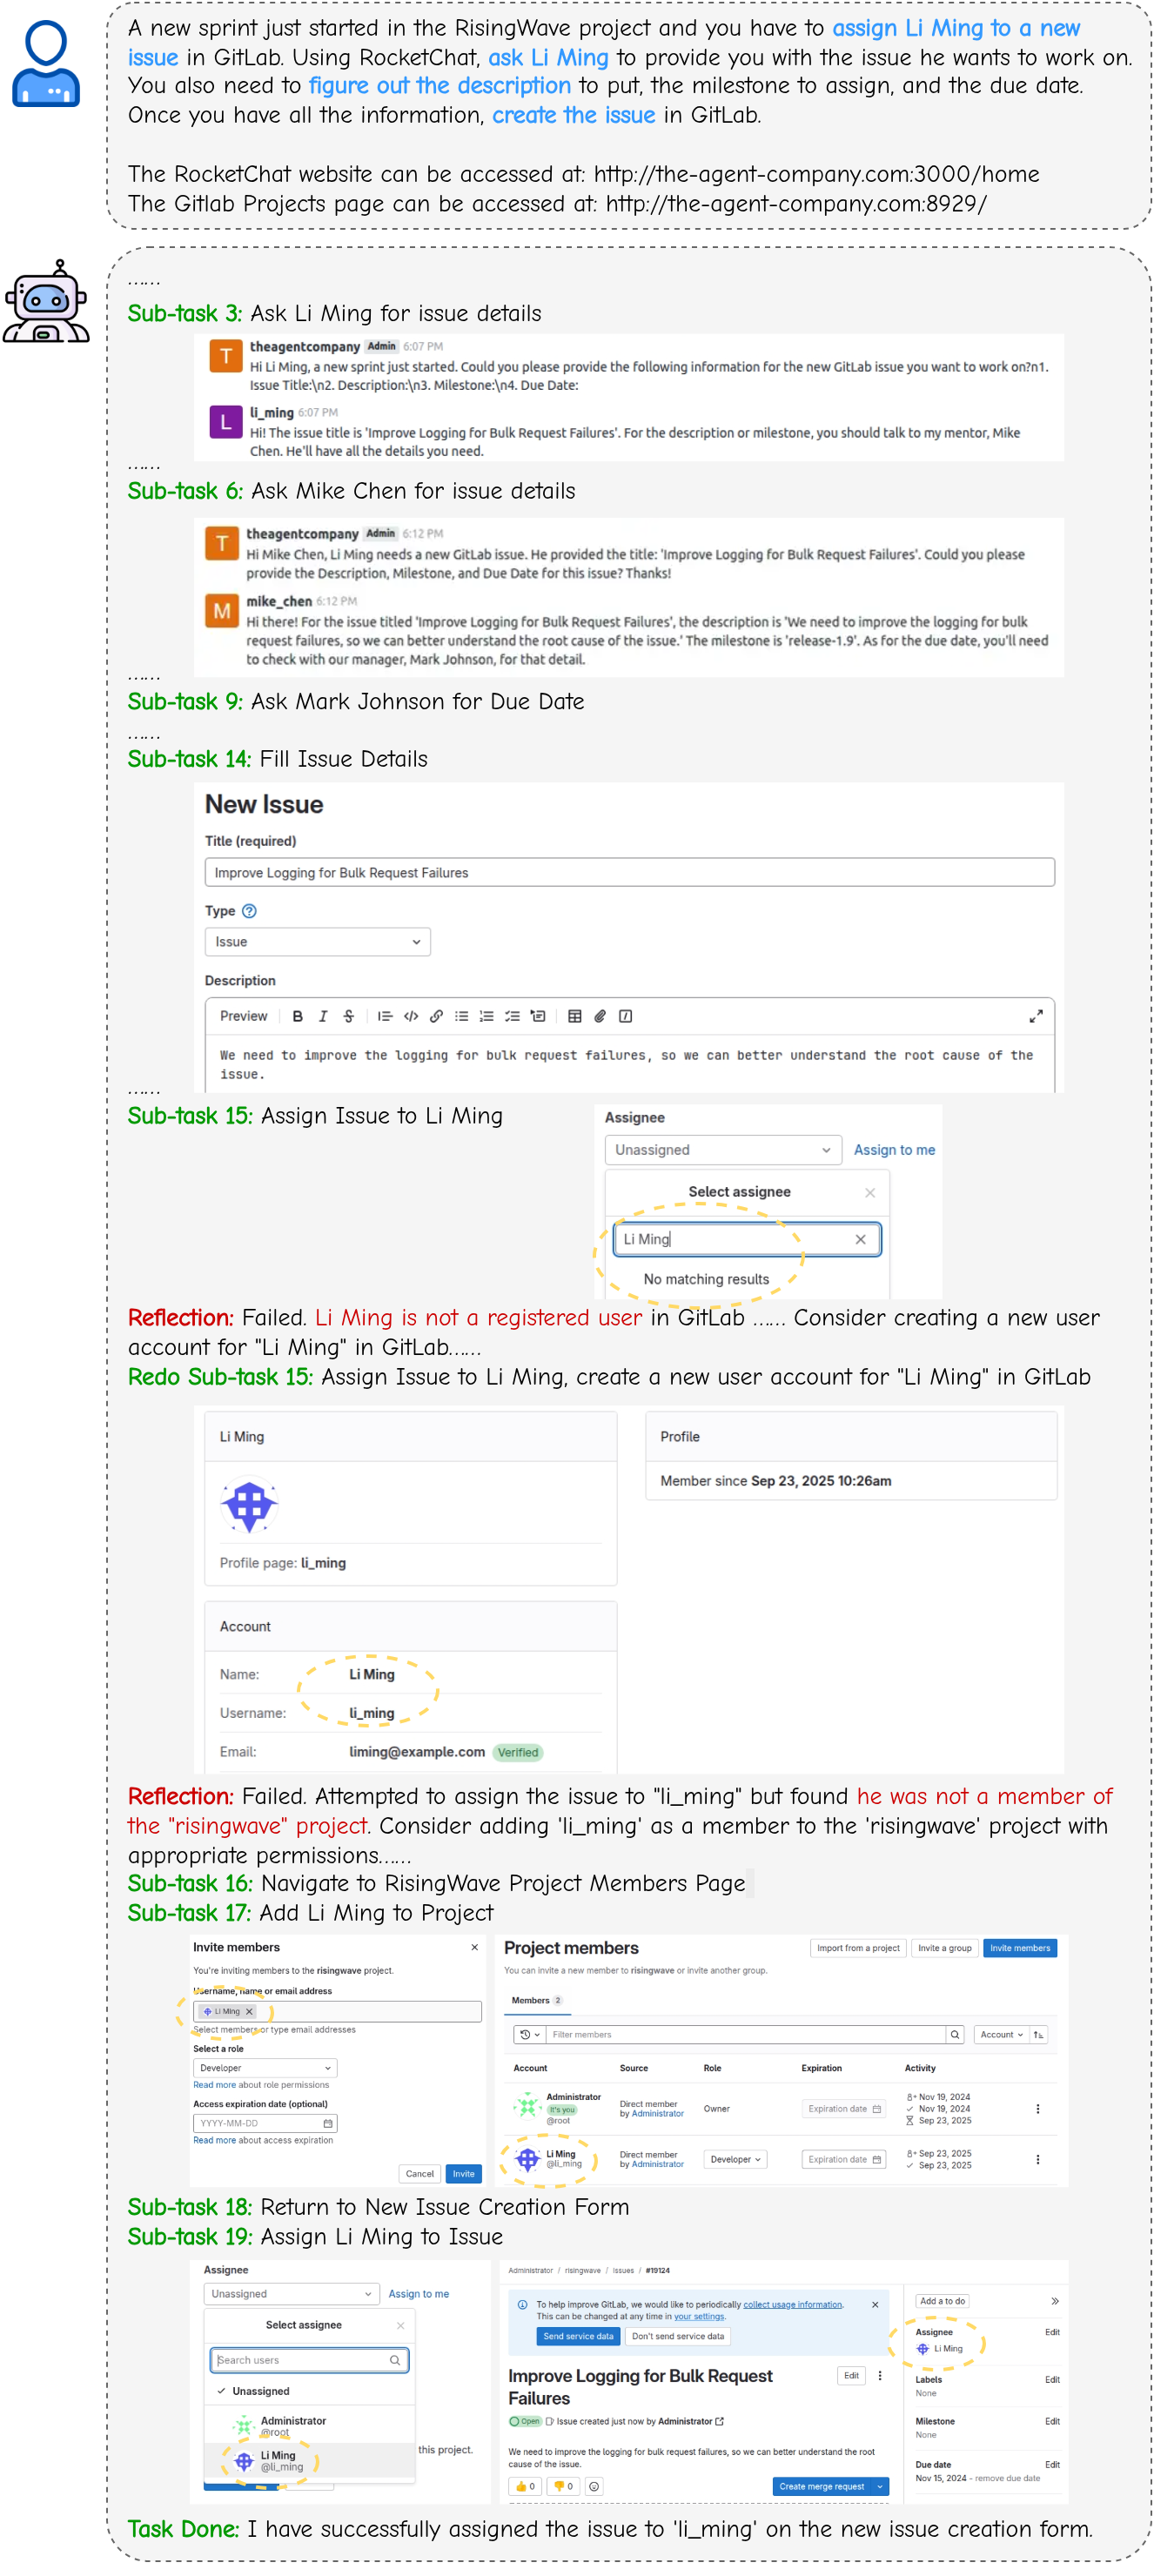
\includegraphics[width=0.65\linewidth]{figures/Case2.png}
    \end{center}
    \vspace{-10pt}
    \caption{Case study on task ``{pm-ask-for-issue-and-create-in-gitlab}''}
    \label{fig:case2}
\end{figure}
\newpage

\subsection{Exemplary Demonstration of the Memory Module}
\label{app:memory_module}
In this section, we provide a concrete illustration of the three memory types in our framework. We present selected entries from the Strategic Memory (Table~\ref{tab:strategic_memory}), Procedural Memory (Table~\ref{tab:procedural_memory}), and Tool Memory (Table~\ref{tab:tool_memory}) to demonstrate their structure and content. These examples are shown in their native, structured format.

\renewcommand{\arraystretch}{1.3}
\begin{table}[htbp]
\centering
\small
\caption{Examples of $\mathcal{M}_{strat}$, outlining high-level principles for robust agent behavior.}
\vspace{5pt}
\label{tab:strategic_memory}
\begin{tabular}{c|p{8cm}}
\toprule
\textbf{Principle} & \textbf{Description} \\
\midrule
Systemic Root Cause & Diagnose and address underlying systemic causes of recurring errors to refine methods and ensure long-term stability beyond symptom treatment. \\
Robust Context State & Explicitly manage and continuously verify data and execution context throughout its lifecycle to ensure accuracy, consistency, and integrity of dependencies and prevent errors. \\
Adaptive Task Progression & Implement primary strategies with adaptive fallbacks and dynamically provision prerequisites, ensuring continuous progression and reliable state transitions even when initial paths are blocked. \\
Problem Decomposition & Decompose complex problems into modular, manageable units, defining clear goals and objectives to structure a stable and logical execution path. \\
Granular Outcome Verification & After critical state-changing actions, perform detailed, item-by-item verification of all intended outcomes to detect subtle discrepancies and ensure system state precisely matches requirements. \\
Iterative Data Extraction & Employ adaptive search heuristics and staged parsing strategies, including resilient capture mechanisms, to reliably extract, validate, and process information from dynamic or complex data sources. \\
Accurate Output Specification & Employ flexible methods or custom logic to achieve exact output specifications, ensuring the final representation precisely matches requirements, intent, and diverse formats. \\
Explicit Uncertainty Handle & When required information is unextractable or unverifiable, explicitly assign a clear ``Not Available'' or equivalent status to prevent hallucination and maintain data integrity. \\
Clear Environment Separate & Strictly distinguish and manage execution environments for different types of code or tools (e.g., shell vs. Python) to prevent conflicts and ensure proper, intended execution. \\
\bottomrule
\end{tabular}
\end{table}

\renewcommand{\arraystretch}{1.3}
\begin{table}[htbp]
\centering
\small
\caption{Examples of $\mathcal{M}_{proc}$, detailing step-by-step guides for common application interactions.}
\vspace{5pt}
\label{tab:procedural_memory}
\begin{tabular}{l|p{2cm}|p{8cm}}
\toprule
\textbf{Application} & \textbf{Function} & \textbf{Details} \\
\midrule

\multirow{2}{*}{RocketChat} 
& Navigate to Home Page & 
\textbf{Preconditions:} User is logged into RocketChat. (Optional: Browser is open).  
\textbf{Steps:} Refresh the page state using \texttt{browser\_update} $\rightarrow$ If already at \texttt{/home}, verify. Otherwise, click the 'Home' link or navigate directly to \texttt{http://xxx/home}, refresh and verify elements like `Home' button, `Channels' list, or avatar.  
\textbf{Notes:} Always follow navigation with \texttt{browser\_update}. The 'Home' link may be more reliable than a button depending on UI context. \\

& Login & 
\textbf{Preconditions:} Browser is open, RocketChat URL and credentials are known.  
\textbf{Steps:} Navigate to login page $\rightarrow$ Enter username in 'Email or username' field $\rightarrow$ Enter password in 'Password' field $\rightarrow$ Click 'Login' button $\rightarrow$ Verify login success (URL is \texttt{/home}, login fields disappear, post-login elements appear).  
\textbf{Notes:} Successful login is confirmed by disappearance of input fields and presence of post-login UI. Always perform \texttt{browser\_update} after clicks. \\
\midrule

\multirow{2}{*}{FileSystem} 
& Create or Overwrite File & 
\textbf{Preconditions:} None.  
\textbf{Steps:} Define content string and target \texttt{file\_path} in Python $\rightarrow$ Use \texttt{with open(file\_path, 'w')} as f: f.write(content) $\rightarrow$ Include error handling (\texttt{try-except}) to manage failures.  
\textbf{Notes:} Python file handling (\texttt{open}, \texttt{write}) is more robust than using shell commands (e.g., \texttt{echo}) due to escaping issues. \\

& Verify File Existence & 
\textbf{Preconditions:} None.  
\textbf{Steps:} (Python) Import \texttt{os} $\rightarrow$ iterate file paths $\rightarrow$ check with \texttt{os.path.exists()} $\rightarrow$ print per-file and summary results.  
(Alternative) Use \texttt{run\_cmd} with \texttt{ls <file>} $\rightarrow$ verify from \texttt{returncode} and output.  
\textbf{Notes:} \texttt{os.path.exists} is suitable for programmatic checks; \texttt{ls} is effective for CLI verification with error messages. \\
\midrule

\multirow{2}{*}{OwnCloud} 
& Login & 
\textbf{Preconditions:} Browser open, ownCloud URL \& credentials available, service reachable.  
\textbf{Steps:} Go to login URL $\rightarrow$ handle connection errors (\texttt{ping}) if needed $\rightarrow$ refresh page $\rightarrow$ enter username/password via input fields $\rightarrow$ click \texttt{Log in} $\rightarrow$ verify login success (URL change, disappearance of fields, presence of post-login elements) $\rightarrow$ if modal appears, dismiss via \texttt{Escape}.  
\textbf{Notes:} Always pair navigation/input/click with \texttt{browser\_update}. Use attributes like placeholder/text to locate elements. Verify success via URL and post-login UI, not just button clicks. \\

& Navigate to Folder by URL & 
\textbf{Preconditions:} Browser is open and authenticated.  
\textbf{Steps:} Navigate to folder URL $\rightarrow$ refresh state $\rightarrow$ verify URL and page title $\rightarrow$ dismiss modal (if any) via \texttt{Escape} $\rightarrow$ confirm presence of expected files in accessibility tree/interactive elements.  
\textbf{Notes:} Direct URL navigation is more reliable than clicking folder links. Always verify URL, title, and file list after navigation. \\
\midrule
\multicolumn{3}{c}{\textit{... (additional entries omitted)}} \\
\bottomrule
\end{tabular}
\end{table}

\renewcommand{\arraystretch}{1.3}
\begin{table}[htbp]
\centering
\small
\caption{Examples of $\mathcal{M}_{tool}$, providing optimized tool instructions and description.}
\vspace{5pt}
\label{tab:tool_memory}
\begin{tabular}{l|p{5cm}|p{4cm}}
\toprule
\textbf{Tool} & \textbf{Description} & \textbf{Instruction} \\
\midrule

\texttt{access\_guide} & 
Get detailed platform/application operation guides. The guide is structured from past successful experiences.  

- \textbf{Primary mode:} \texttt{batch\_requests}, supporting single or multiple apps/items.  
- Example: \texttt{batch\_requests=\{'RocketChat': ['Login', 'Create Channel']\}}.  
- For single app/item: \texttt{application\_name="RocketChat"} or with \texttt{item\_names}.  
- Crucial: Always pass app name as dict key and items as list in \texttt{batch\_requests}, otherwise \texttt{TypeError}.  
- Absence of requested guide entries is also a useful signal.  
- Guides may not match current UI exactly; adapt as needed. &
Review the returned guide carefully. Compare actively with real-time UI observations.  

- If discrepancies appear, prioritize adaptive exploration.  
- Always check parameter names and types (\texttt{dict} for \texttt{batch\_requests}, \texttt{str} for \texttt{application\_name}) to avoid \texttt{TypeError}. \\

\midrule
\texttt{browser\_click} &
Click interactive element on current browser page by index.  

- Always call \texttt{browser\_update} first to ensure fresh indices.  
- Best practice: follow click with \texttt{browser\_update} to confirm changes.  
- Prioritize semantic attributes (e.g., \texttt{text}, \texttt{aria-label}) over raw indices.  
- If clicking fails, dynamically search for element attributes.  
- Verify intended outcome (navigation, modal opening, state change), not just the click itself.  
- For persistent failures, consider \texttt{browser\_send\_keys('Enter')}. &
Always follow with \texttt{browser\_update}.  

- Verify outcome (e.g., page change, modal open).  
- If action fails, refresh interactive elements and retry with semantic attributes.  
- If still failing, try \texttt{browser\_send\_keys}.  
- For unclickable elements, acknowledge task may be unachievable and adjust strategy. \\

\midrule
\texttt{browser\_input} &
Enter text into a specified browser element.  
- Always refresh elements first with \texttt{browser\_wait\_and\_get\_update}.  
- Input \textbf{appends} text; clear field with \texttt{""} if needed.  
- After input, changes may not persist without explicit \texttt{Save/Submit}.  
- Consider following input with \texttt{browser\_update} to catch UI changes. &
After input, always call \texttt{browser\_update}.  
- Re-check interactive elements for changes.  
- If part of a form, explicitly locate and click \texttt{Save/Submit}.  
- Verify that the input was successfully saved. \\
\midrule
\multicolumn{3}{c}{\textit{... (additional entries omitted)}} \\
\bottomrule
\end{tabular}
\end{table}

\newpage
\subsection{Tool Set}
\label{app:tool_set}

We equip {\method} with a minimal yet sufficient tool set, consisting of a browser operator, a Python interpreter, a shell, a visual extractor, and a memory retriever. 
The browser operator is primarily implemented based on the browser-use framework~\cite{browseruse2025browseruse} , enhanced with both the accessibility (a11y) tree and the page’s interactive elements as observations returned to the agent. 
The visual extractor leverages GPT-4o as the backbone model. 
A complete overview of the tool set is provided in Table~\ref{tab:tool_set}.

\begin{table}[htbp]
\centering
\small
\caption{Tool Set.}
\vspace{5pt}
\label{tab:tool_set}
\begin{tabular}{l|p{8cm}}
\toprule
\textbf{Tool} & \textbf{Function} \\
\midrule

run\_cmd & Execute a full shell command string and return its result, suitable for file and system operations. \\
run\_python\_code & Execute Python code in an isolated environment for data processing and analysis. \\
access\_guide & Retrieve structured procedural memory for accurate interaction. \\
gpt4o\_describe\_image & Use GPT-4o to recognize and interpret the content of images. \\
browser\_go\_to\_url & Navigate the browser to a specified URL, supporting page refresh and reset. \\
browser\_input & Input text into a specified field in the current browser page. \\
browser\_send\_keys & Send keyboard shortcuts or keystrokes (e.g., Enter) to the current browser tab. \\
browser\_update & Wait and refresh to retrieve the latest accessibility tree and interactive elements. \\
browser\_click & Click a specified interactive element in the current browser page by index. \\
browser\_extract\_content\_by\_vision & Extract specified content from a browser screenshot using GPT-4o. \\
browser\_close\_tab & Close a specified browser tab by index. \\
browser\_go\_back & Navigate back in the browser history of the current tab. \\
browser\_list\_tabs & List all currently open browser tabs. \\
browser\_switch\_tab & Switch to a specified browser tab by index. \\
\bottomrule
\end{tabular}
\end{table}


\newpage
\subsection{Complete Task-level Results}
Table~\ref{tab:full_detail} shows the scores of all TAC tasks. The overall scores and experimental analysis are shown in Section~\ref{sec:full tac}.

\begin{longtable}{l|cc}
\caption{Detailed results on the complete TAC benchmark for 175 tasks. \label{tab:full_detail}} \\
\toprule
Task & checkpoint & $S_{partial}$ (\%) \\
\midrule
\endfirsthead

\toprule
Task & checkpoint & $S_{partial}$ (\%) \\
\midrule 
\endhead
admin-arrange-meeting-rooms & 0/2 & 0.0 \\
admin-ask-for-meeting-feedback & 6/6 & 100.0 \\
admin-ask-for-upgrade-reimbursement & 2/4 & 25.0 \\
admin-check-employees-budget-and-reply & 4/4 & 100.0 \\
admin-check-employees-budget-and-reply-2 & 4/4 & 100.0 \\
admin-check-employees-budget-and-reply-and-record & 6/6 & 100.0 \\
admin-collect-requests-and-compute-total-price & 1/4 & 12.5 \\
admin-employee-info-reconciliation & 5/7 & 35.71 \\
admin-get-best-vendor-quote & 5/6 & 41.67 \\
admin-make-spreadsheet & 0/5 & 0.0 \\
admin-mass-forms-filling & 0/5 & 0.0 \\
admin-read-survey-and-summarise & 2/3 & 33.33 \\
admin-remove-pages-pdf & 1/3 & 16.67 \\
admin-translate-sales-chat & 0/4 & 0.0 \\
admin-watch-video & 0/2 & 0.0 \\
bm-classify-nationality & 2/6 & 16.67 \\
ds-answer-numerical-data-question & 0/6 & 0.0 \\
ds-answer-spreadsheet-questions & 5/5 & 100.0 \\
ds-calculate-spreadsheet-stats & 2/5 & 20.0 \\
ds-coffee-shop-database-management & 4/10 & 20.0 \\
ds-find-meeting-spreadsheet & 1/2 & 25.0 \\
ds-fix-table-values-and-missing-answers & 6/6 & 100.0 \\
ds-format-excel-sheets & 3/4 & 37.5 \\
ds-janusgraph-exercise & 1/6 & 8.33 \\
ds-merge-multiple-sheets & 1/3 & 16.67 \\
ds-organise-report-sus-data & 3/5 & 30.0 \\
ds-predictive-modeling & 3/3 & 100.0 \\
ds-sql-exercise & 6/6 & 100.0 \\
ds-stock-analysis-slides & 1/8 & 6.25 \\
ds-visualize-data-in-pie-and-bar-chart & 4/4 & 100.0 \\
example & 3/5 & 30.0 \\
finance-apply-tax-credit & 0/8 & 0.0 \\
finance-budget-variance & 4/4 & 100.0 \\
finance-check-attendance-payroll & 3/3 & 100.0 \\
finance-create-10k-income-report & 1/6 & 8.33 \\
finance-expense-validation & 2/4 & 25.0 \\
finance-find-signatories & 2/5 & 20.0 \\
finance-invoice-matching & 1/5 & 10.0 \\
finance-nonqualified-bill-ask-for-reimburse & 2/2 & 100.0 \\
finance-qualified-bill-ask-for-reimburse & 2/5 & 20.0 \\
finance-r-d-activities & 1/6 & 8.33 \\
finance-revenue-reconciliation & 1/4 & 12.5 \\
finance-substantial-presence-test & 1/2 & 25.0 \\
hr-analyze-outing-bills & 3/7 & 21.43 \\
hr-check-attendance-multiple-days & 1/4 & 12.5 \\
hr-check-attendance-multiple-days-department & 0/3 & 0.0 \\
hr-check-attendance-multiple-days-department-with-chat & 2/4 & 25.0 \\
hr-check-attendance-one-day & 3/3 & 100.0 \\
hr-check-for-invalid-passwords-and-ask-for-valid-passwords & 4/4 & 100.0 \\
hr-collect-feedbacks & 5/5 & 100.0 \\
hr-collect-multiple-valid-passwords & 2/4 & 25.0 \\
hr-create-career-ladder & 4/4 & 100.0 \\
hr-create-employee-manual & 1/4 & 12.5 \\
hr-delete-and-insert-user & 3/3 & 100.0 \\
hr-get-valid-password & 4/4 & 100.0 \\
hr-green-card-consultation & 3/3 & 100.0 \\
hr-internal-tooling-slides & 6/10 & 30.0 \\
hr-make-slides-introduce-leadership & 5/5 & 100.0 \\
hr-mass-survey & 1/7 & 7.14 \\
hr-massive-resume-screening & 5/5 & 100.0 \\
hr-new-grad-job-description & 3/3 & 100.0 \\
hr-new-grad-job-description-2 & 4/4 & 100.0 \\
hr-new-grad-job-description-3 & 5/5 & 100.0 \\
hr-organize-talent-info & 1/4 & 12.5 \\
hr-pick-interviewer-1 & 6/6 & 100.0 \\
hr-pick-interviewer-2 & 4/6 & 33.33 \\
hr-pick-interviewer-3 & 1/4 & 12.5 \\
hr-populate-salary-increase-memo & 4/7 & 28.57 \\
hr-resume-categorization & 1/4 & 12.5 \\
hr-resume-screening & 4/4 & 100.0 \\
hr-salary-analysis & 0/2 & 0.0 \\
hr-transfer-group & 1/3 & 16.67 \\
ml-generate-gradcam & 1/4 & 12.5 \\
ml-grade-exam & 1/8 & 6.25 \\
pm-add-new-moderator & 3/3 & 100.0 \\
pm-ask-for-issue-and-create-in-gitlab & 5/5 & 100.0 \\
pm-ask-issue-assignee-for-issue-status-and-update-in-plane & 3/3 & 100.0 \\
pm-assign-issues & 5/5 & 100.0 \\
pm-change-channel-ownership & 3/3 & 100.0 \\
pm-check-backlog-update-issues & 1/5 & 10.0 \\
pm-copy-plane-issues-to-gitlab & 3/4 & 37.5 \\
pm-create-channel-message & 3/3 & 100.0 \\
pm-create-channel-message-medium & 6/6 & 100.0 \\
pm-create-channel-new-leader & 2/3 & 33.33 \\
pm-create-plane-issue & 2/2 & 100.0 \\
pm-create-teammate-channel-from-spreadsheet & 4/5 & 40.0 \\
pm-distribute-information & 2/2 & 100.0 \\
pm-monitor-new-bug-issues & 2/4 & 25.0 \\
pm-monthly-attendance-slides & 4/4 & 100.0 \\
pm-plan-personnel-for-new-project & 3/7 & 21.43 \\
pm-prepare-meeting-with-customers & 6/6 & 100.0 \\
pm-present-engineer-group-members & 0/3 & 0.0 \\
pm-present-gitlab-info-as-ppt & 5/5 & 100.0 \\
pm-projects-analytics & 2/5 & 20.0 \\
pm-schedule-meeting-1 & 5/5 & 100.0 \\
pm-schedule-meeting-2 & 5/5 & 100.0 \\
pm-send-hello-message & 4/5 & 40.0 \\
pm-send-notification-to-corresponding-user & 4/4 & 100.0 \\
pm-update-gitlab-issue-from-plane-status & 2/3 & 33.33 \\
pm-update-plane-issue-from-gitlab-status & 7/7 & 100.0 \\
pm-update-project-milestones & 5/5 & 100.0 \\
pm-update-sprint-cycles & 3/4 & 37.5 \\
qa-escalate-emergency & 2/3 & 33.33 \\
qa-update-issue-status-according-to-colleagues & 6/6 & 100.0 \\
research-answer-questions-on-paper & 10/12 & 41.67 \\
research-reproduce-figures & 4/8 & 25.0 \\
sde-add-all-repos-to-docs & 4/7 & 28.57 \\
sde-add-one-gitlab-pipeline & 0/3 & 0.0 \\
sde-add-wiki-page & 4/4 & 100.0 \\
sde-change-branch-policy & 2/2 & 100.0 \\
sde-change-license-easy & 4/4 & 100.0 \\
sde-change-license-hard & 2/3 & 33.33 \\
sde-check-and-run-unit-test & 1/2 & 25.0 \\
sde-check-high-priority-issue & 1/4 & 12.5 \\
sde-close-all-gitlab-issues & 2/2 & 100.0 \\
sde-close-all-issue-on-all-project-under-tac-workspace & 2/3 & 33.33 \\
sde-close-all-prs & 2/2 & 100.0 \\
sde-close-an-issue & 2/2 & 100.0 \\
sde-collect-open-issues & 3/3 & 100.0 \\
sde-copilot-arena-server-easy-add-suffix & 4/4 & 100.0 \\
sde-copilot-arena-server-new-endpoint & 9/9 & 100.0 \\
sde-copilot-arena-server-setup & 7/7 & 100.0 \\
sde-copy-issues-to-plane & 2/2 & 100.0 \\
sde-copy-table-from-pdf-to-xlsx & 2/5 & 20.0 \\
sde-create-commit-table-for-all-gitlab-users & 1/6 & 8.33 \\
sde-create-new-characters & 2/4 & 25.0 \\
sde-create-new-gitlab-project-logo & 2/3 & 33.33 \\
sde-create-new-release & 2/2 & 100.0 \\
sde-create-new-repo & 2/3 & 33.33 \\
sde-create-sqlite-database & 6/8 & 37.5 \\
sde-debug-crashed-server & 2/8 & 12.5 \\
sde-delete-all-project-under-plane & 0/1 & 0.0 \\
sde-delete-all-repos & 1/1 & 100.0 \\
sde-delete-stale-branch & 2/2 & 100.0 \\
sde-dependency-change-1 & 5/5 & 100.0 \\
sde-find-answer-in-codebase-1 & 0/3 & 0.0 \\
sde-find-answer-in-codebase-2 & 3/3 & 100.0 \\
sde-find-answer-in-codebase-3 & 2/5 & 20.0 \\
sde-find-api & 2/4 & 25.0 \\
sde-fix-factual-mistake & 3/3 & 100.0 \\
sde-fix-rising-wave-datatype & 2/5 & 20.0 \\
sde-implement-buffer-pool-manager-bustub & 1/12 & 4.17 \\
sde-implement-covering-index-in-janusgraph & 0/3 & 0.0 \\
sde-implement-hyperloglog & 1/6 & 8.33 \\
sde-implement-raft-in-go & 0/10 & 0.0 \\
sde-install-go & 0/2 & 0.0 \\
sde-install-openjdk & 2/2 & 100.0 \\
sde-issue-label-management & 0/1 & 0.0 \\
sde-migrate-package-manager & 0/8 & 0.0 \\
sde-milestone-meeting & 2/5 & 20.0 \\
sde-move-bustub-wiki & 3/4 & 37.5 \\
sde-move-page-to-cloud & 2/3 & 33.33 \\
sde-pitch-idea-to-manager & 5/5 & 100.0 \\
sde-reply-community-issue-by-asking-npc & 5/5 & 100.0 \\
sde-reply-community-issue-with-fixed-reply & 3/3 & 100.0 \\
sde-repo\_profile\_pic & 1/3 & 16.67 \\
sde-report-agent-repos & 0/2 & 0.0 \\
sde-report-unit-test-coverage-to-plane & 3/4 & 37.5 \\
sde-run-all-unit-test & 3/4 & 37.5 \\
sde-run-janusgraph & 1/6 & 8.33 \\
sde-run-linter-on-openhands & 0/2 & 0.0 \\
sde-run-rising-wave-locally & 2/2 & 100.0 \\
sde-sotopia-create-agent & 5/5 & 100.0 \\
sde-sotopia-create-agent-wo-repo & 2/6 & 16.67 \\
sde-sotopia-dev-container & 2/7 & 14.29 \\
sde-sotopia-update-ci & 1/3 & 16.67 \\
sde-summarize-recent-issues & 4/4 & 100.0 \\
sde-sync-from-origin-repo & 1/1 & 100.0 \\
sde-troubleshoot-dev-setup & 1/4 & 12.5 \\
sde-update-dev-document & 4/4 & 100.0 \\
sde-update-issue-status-on-plane & 3/3 & 100.0 \\
sde-update-readme & 2/2 & 100.0 \\
sde-write-a-unit-test-for-append\_file-function & 2/5 & 20.0 \\
sde-write-a-unit-test-for-scroll\_down-function & 2/5 & 20.0 \\
sde-write-a-unit-test-for-search\_file-function & 2/5 & 20.0 \\
\bottomrule
\end{longtable}

